\documentclass[12pt,a4paper]{report}

\newcommand{\studentNameone}{Student Full Name}
\newcommand{\studentNametwo}{Student Full Name}
\newcommand{\studentNamethree}{Student Full Name}
\newcommand{\studentNamefour}{Student Full Name}
\newcommand{\guideName}{Mr. Guide Name}
\newcommand{\headName}{Mr. Head Name}
\newcommand{\enrollmentNumberone}{20XX02100XX000X}
\newcommand{\enrollmentNumbertwo}{20XX02100XX000X}
\newcommand{\enrollmentNumberthree}{20XX02100XX000X}
\newcommand{\enrollmentNumberfour}{20XX02100XX000X}
\newcommand{\reportTitle}{Seminar Report Title}
\newcommand{\instituteName}{Chhotubhai Gopalbhai Patel Institute of Technology}
\newcommand{\instituteNameshort}{CGPIT}
\newcommand{\degreeName}{Diploma}
\newcommand{\branchName}{Branch Name}
\newcommand{\departmentName}{Department of CE/IT }
\newcommand{\locationName}{Bardoli, Surat}
\newcommand{\universityName}{Uka Tarsadia University}
\newcommand{\academicYear}{April-2019}


\usepackage[pdftex]{graphicx}
%\DeclareGraphicsExtensions{.pdf,.jpeg,.png}
\usepackage{graphicx} %for including images
\usepackage{setspace} %for line spacing
\usepackage{tabularx} %for basic spacing in caption and table
\renewcommand{\baselinestretch}{1.5}

\usepackage[pages=some]{background} %to add watermark
\backgroundsetup{                      %to add watermark
contents={
\includegraphics{UTU.png}},
angle=0,
scale=4,
color=black,
opacity=0.2
}

\usepackage{tocloft}    % tocloft for table of contents style

\usepackage[compact]{titlesec}  % titlesec for title section layout
\newcommand*{\justifyheading}{\raggedleft} % for right justification of chapters

%remove space before chapter title
\titleformat{\chapter}[display]
{\normalfont\huge\bfseries\justifyheading}{\chaptertitlename\ \thechapter}{20pt}{\Huge}
\titlespacing*{\chapter}{0pt}{-50pt}{40pt}


\renewcommand{\contentsname}{
\begin{center}
\LARGE\bf TABLE OF CONTENTS
\end{center}
} %for changing the contents title

\renewcommand\listtablename{
\begin{center}
\LARGE\bf LIST OF TABLES
\end{center}
} %for changing list of table title

\renewcommand\listfigurename{
\begin{center}
\LARGE\bf LIST OF FIGURES
\setlength\cftbeforefigskip{\cftbeforechapskip}
\end{center}
} %for changing list of figure title

\usepackage{subfig}

\renewcommand\cftchapafterpnum{\vskip6pt}   %for spacing change in table of content
\renewcommand\cftsecafterpnum{\vskip10pt}   %for spacing change in table of content
\renewcommand\cftsubsecafterpnum{\vskip10pt}
\renewcommand\cftsubsubsecafterpnum{\vskip10pt}

%--------------parth------------
\usepackage{color}   %May be necessary if you want to color links
\usepackage{hyperref}
\hypersetup{
    linktoc=all,     %set to all if you want both sections and subsections linked
    linkcolor=black  %choose some color if you want links to stand out
}
\usepackage{url}
\usepackage{notoccite}
\usepackage{float}
\usepackage{pdflscape}

%\usepackage{indentfirst }
%\usepackage{subcaption}
%%%%% For Removing paragraph
\setlength\parindent{0pt}

\usepackage{enumerate}
\newenvironment{tight_enumerate}{
 \begin{enumerate}
 \setlength{\topsep}{0pt}
 \setlength{\itemsep}{0pt}
 \setlength{\parskip}{0pt} }
{\end{enumerate}
}

\newenvironment{tight_itemize}{
 \begin{itemize}
 \setlength{\topsep}{0pt}
 \setlength{\itemsep}{0pt}
 \setlength{\parskip}{0pt} }
{\end{itemize}
}


\newenvironment{tight_description}{
 \begin{description}
 \setlength{\topsep}{0pt}
 \setlength{\itemsep}{0pt}
 \setlength{\parskip}{0pt} }
{\end{description}
}

%-----------------parth end----------------
%------------------------- Document settings ------------------------
\topmargin   0mm
\hoffset     0mm
\voffset     0mm
\textwidth   155mm
\textheight  230mm
%------------------------- Definitions ------------------------------



%------------------------- document ---------------------------------

\begin{document}
% --------- Title and abstract etc the front matter -----------
\pagenumbering{roman}
% TITLE PAGE

\thispagestyle{empty}

\begin{center}

{\large {A seminar report on}}
\vspace{0.6cm}

{\Huge \textbf{\reportTitle}}
\vspace{0.6cm}

{\large\textbf{by}}\\
{\large \bf \studentNameone} 
{\bf (\enrollmentNumberone)}\\
{\large \bf \studentNametwo} 
{\bf (\enrollmentNumbertwo)}\\
{\large \bf \studentNamethree} 
{\bf (\enrollmentNumberthree)}\\
{\large \bf \studentNamefour} 
{\bf (\enrollmentNumberfour)}\\
\vspace{0.9cm}

in Partial Fulfilment of the Requirements for the Degree of
\vspace{0.6cm}


{\large\textbf{\degreeName}}\\
{\large{in}}\\
{\large\textbf{\branchName}}\\
\vspace{0.9cm}
{\large{at}}\\
{\Large \textbf{UKA TARSADIA UNIVERSITY}}
\vspace{0.6cm}

{\large\textbf{Under the guidance of}}\\
{\large \bf \guideName}
\vspace{0.2cm}

\begin{figure}[h]
\begin{center}
 
\includegraphics[scale=0.8]{UTU.png}
\end{center}
\end{figure}
{\bf \departmentName}\\
{\bf \instituteName}\\
{\bf \locationName}\\
{\bf \academicYear}
\end{center}

% -------------------------------------------------------------------------
\newpage
\addcontentsline{toc}{chapter}{CERTIFICATE}
\BgThispage

\begin{center}
{\LARGE \bf CERTIFICATE}\\
\end{center}
\vspace{0.8cm}
%\fontsize{12pt}{20pt}\selectfont
This is to certify that the seminar report entitled ``\textbf{\reportTitle}" has been carried out by \textbf{\studentNameone (\enrollmentNumberone)}, \textbf{\studentNametwo (\enrollmentNumbertwo)}, \textbf{\studentNamethree (\enrollmentNumberthree)}, \textbf{\studentNamefour (\enrollmentNumberfour)} at \textbf{\instituteName} for the partial fulfillment of \degreeName in \branchName degree to be awarded by \textbf{UKA TARSADIA UNIVERSITY}.
\\
\\
\textbf{Date:}\\
\textbf{Place:} \locationName\\
\\
\\
\\
\\
\\
\\
\\
\\
\\
\\
\begin{tabular}{l l l}
\noindent \guideName  & \hspace{5cm} & \headName \\
Guide, &  & Head,\\
\departmentName,& & \departmentName,\\
\instituteNameshort& &\instituteNameshort \\
\end{tabular}
\\
\\
\\
\begin{center}
  Examiner's Signature
\end{center}
% -------------------------------------------------------------------------
\newpage
\addcontentsline{toc}{chapter}{ACKNOWLEDGEMENT}
\begin{center}
{\LARGE \bf ACKNOWLEDGEMENT}\\
\end{center}
\vspace{0.8cm}

I have taken efforts in this seminar work. However, it would not have been possible
without the kind support and help of many individuals. I would like to extend my sincere thanks to all of them.

I am highly indebted to \textbf{\guideName} for his guidance and constant supervision as well as for providing necessary information regarding the seminar work.

I would like to express my gratitude towards my parents and member of family for their kind co-operation and encouragement which help me in completion of this project.
My thanks and appreciations also go to people who have willingly helped me out with
their abilities.


\begin{flushright}
\textbf{\studentNameone}\\
\textbf{\studentNametwo}\\
\textbf{\studentNamethree}\\
\textbf{\studentNamefour}
\end{flushright}


%---------------------------------------------------------------------------
\newpage
\addcontentsline{toc}{chapter}{ABSTRACT}
\begin{center}
{\LARGE \bf ABSTRACT}\\
\end{center}
\vspace{0.8cm}

\emph{Virtualization is a method of running multiple independent virtual operating systems
on a single physical computer. All the guest operating systems are completely isolated
It is a way of maximizing utilization of physical resources in order to minimize
investment in hardware. It also increase total productivity of the hardware. It has
been around since the first mainframe systems. This seminar mainly focuses on
virtualization as it pertains in any organization, but before considering any type of
server virtualization, it's important to define what technology or category of service
you're trying to virtualizes. Generally speaking, virtualization falls into three
categories: Operating System, Network, and Applications. All these categories
depends on one other. We can achieve scalability , reduce cost and reduce risk of
failure.}

%---------------------------------------------------------------------------



\begin{singlespace}


\newpage
\setlength{\cftbeforetoctitleskip}{-4em}  %for removing space before table of content title
\tableofcontents
\newpage
\addcontentsline{toc}{chapter}{LIST OF TABLES}
\setlength{\cftbeforelottitleskip}{-4em}  %for removing space before list of tables title
\listoftables
\newpage
\addcontentsline{toc}{chapter}{LIST OF FIGURES}
\setlength{\cftbeforeloftitleskip}{-4em}   %for removing space before list of figures title
\listoffigures
\end{singlespace}

\newpage
\addcontentsline{toc}{chapter}{LIST OF ABBREVIATIONS}\index{Abbreviations}
%\listofabbrevations
\begin{center}
{\LARGE \bf LIST OF ABBREVIATIONS}\\
\end{center}
\vspace{1.6cm}
AI \dotfill Artificial Intelligence\\
ANN \dotfill Artificial Neural Networks\\
BLEU \dotfill Bilingual Evaluation Understudy\\
CNN \dotfill Convolutional Neural Networks\\
%DIGITS \dotfill Deep Learning GPU Training System\\
GPU \dotfill Graphics Processing Unit\\
%ILVRC \dotfill ImageNet Large Scale Visual Recognization Challange\\
LSTM \dotfill Long Short Term Memory\\
MNIST \dotfill Mixed National Institute of Standards and Technology\\
NIST \dotfill National Institute of Standards and Technology\\
NN \dotfill Neural Network\\
NMT \dotfill Neural Machine Translation\\
RNN \dotfill Recurrent Neural Network\\


\newpage
\pagenumbering{arabic}
\pagestyle{headings}
% ----------------- thesis chapters -----------
% ----Introduction----------
\flushbottom
\chapter{Introduction}\label{Introduction}
Even before computer's invention, inventors have dreamed of creating machine that can think like human. More than 100 years before first programmable computer was actually built, people wondered whether such machines might become intelligent.\\

Today, Artificial Intelligence (AI) is one of the very active area of research with huge amount of practical applications.
We are applying smart and intelligent system everywhere like automating routine tasks, understand speech or images, make diagnoses in medicine and support basic scientific research.

\section{Machine Learning}
 In early days, computers were mainly used for solving problems that are intellectually difficult for human beings but relatively straightforward for computers which can be described by list of formal or mathematical rules. But main challenge is to solve real world tasks that are very easy to perform by human but hard to describe by rule or equation like recognizing spoken words or identifying objects in images.\\

 The difficulties faced by systems relying on hard-coded knowledge suggest that AI systems need the ability to acquire their own knowledge, by extracting patterns from raw data. This capability is known as machine learning. We can formally define machine learning as ``A computer program is said to learn from experience E with respect to some class of tasks T and performance measure P, if its performance at tasks in T, as measured by P, improves with  experience E" .\\

 The introduction of machine learning allowed computers to tackle problems involving knowledge of the real world and make decisions that appear subjective.
 Machine learning is conceptualized as a part of whole  artificial intelligence ecosystem. As you can see in Figure \ref{MLNNDL} a more specialized branch of machine learning is using neural networks as its building blocks.

\begin{figure}[h]
  \centering
  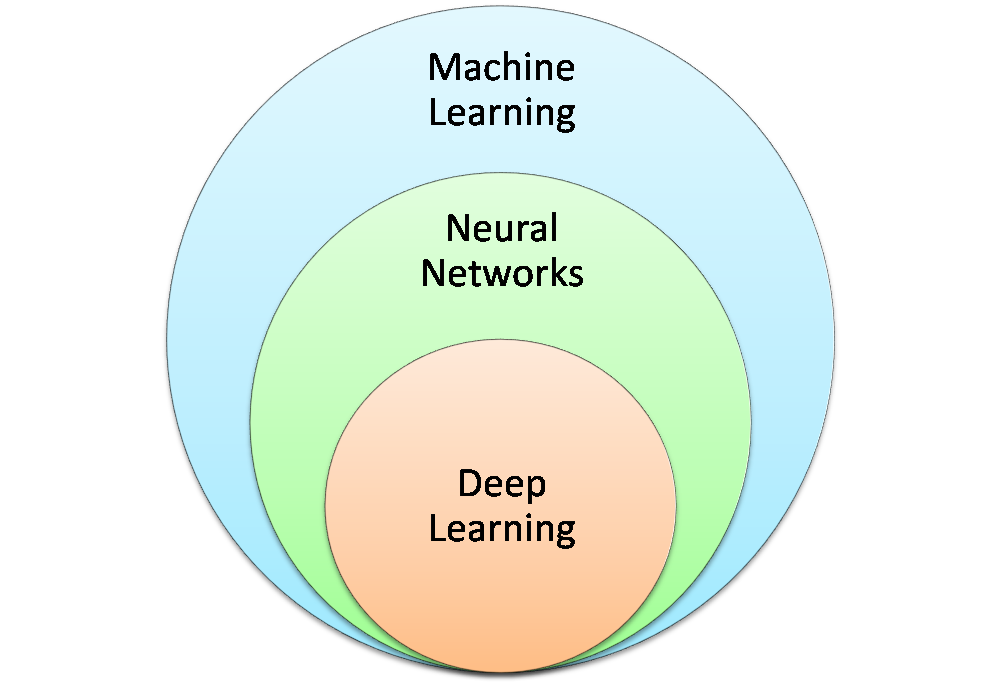
\includegraphics[width=13cm]{img/MLNNDL}
  \caption{Hierarchy of machine learning}\label{MLNNDL}
\end{figure}

 The performance of simple machine learning algorithms depends heavily on the representation of the data they are given. This dependence on representations is a general phenomenon that appears throughout computer science. The choice of representation has an enormous effect on the performance of machine learning algorithms. Once we identify what features to extract, we can teach machine to learn pattern using these features. These tasks can be done using artificial neural networks. By combining multiple neurons we can create artificial neural network which can be trained to perform any given task.\\

As we can see in Figure \ref{learningsteps} process of learning can be divided in two parts:
\begin{tight_enumerate}
  \item Training
  \item Inference
\end{tight_enumerate}

  \begin{figure}[H]
  \centering
  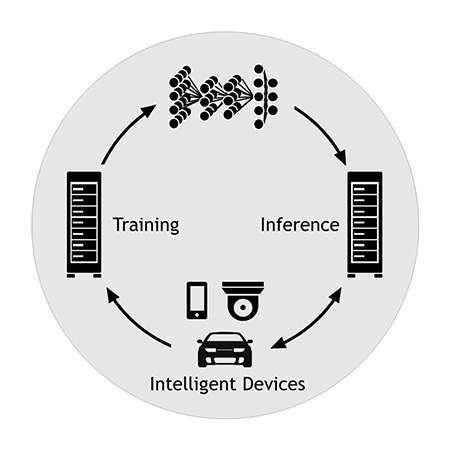
\includegraphics[width=10cm]{img/steps}
  \caption[Steps of learning]{Steps of learning \cite{GTCx}}\label{learningsteps}
\end{figure}

\section{Deep Learning}

Concept of deep learning is nothing new. It was introduced way back in early 80's when computers were not even in day to day usage. First paper on LeNet, a deep convolutional neural network was published in 1989 by Y. LeCun. But back than there was not enough environment available for development of deep neural networks. But recent advancement in field of machine learning started only since 2012 when Alex Krizhevsky successfully demonstrated use of convolutional neural networks by beating traditional methods in ImageNet Large Scale Visual Recognition challenge (ILSVRC) by large margin. This was only possible due to 3 main things \cite{Gettingstartdeeplearninig}:

\begin{itemize}
  \item Use of deep neural network with large number of hidden layer.
  \item Availability of huge amount of data to use for training.
  \item Availability of high performance computing power using GPU.
\end{itemize}

 Ironically, abstract and formal tasks that are among the most difficult mental undertakings for a human being are among the easiest for a computer. From the long time computers have able to defeat the best human chess player, but only recently they are matching some of the abilities of average human beings to recognize objects or speech. A person's everyday life requires an immense amount of knowledge about the world. Much of this knowledge is subjective and intuitive, and therefore difficult to articulate in a formal way. Computers need to capture this same knowledge in order to behave in an intelligent way. One of the key challenges in artificial intelligence is how to get this informal knowledge into a computer.

\section{Benefits of using Deep Learning}
Deep learning is considered as best way to make machine intelligent due to some of following benefits \cite{Gettingstartdeeplearninig}:
\subsection{Robust}
Deep neural networks learn automatically. There is no need to design the features ahead of time. Features are automatically learned to be optimal for specified task.
\subsection{Generalizable}
Same neural network approach can be used in many different applications and different data types for example same network that we use for image labeling can be used for character recognition.
\subsection{Scalable}
Compared to other types of learning performance of deep learning networks improves with more data. These networks are also highly parallelizable due to high number of independent mathematical operations.

\flushbottom
%%-------------------------------------------------------------------------
% ----Literature Review---------
\flushbottom
\chapter{Brief Overview}\label{Brief Overview}
\section{Background}
To perform task of image captioning we need to first identify objects in an image. That can be done using one of the image labeling model given in next section. These image labeling models generally contains combination of one or more than one types of neural networks which we have discussed in this chapter. Once objects are detected we will generate caption using any of image captioning model.
\section{Different types of neural networks}
Image labeling models are deep learning models that are designed specifically for identifying objects in an image and generate labels based on objects in an image.
\subsection{Recurrent Neural Network (RNN)}

The idea behind RNNs is to make use of sequential information. In normal feedforward networks there is a single input which completely determines the activations of all the neurons through the remaining layers. But if we modify it in such a way that the behaviour of hidden neurons might not just be determined by the activations in previous hidden layers, but also by the activations at earlier times. Indeed, a neuron's activation might be determined in part by its own activation at an earlier time. 

 Here is what a typical RNN looks like:

\begin{figure}[h]
\begin{center}
     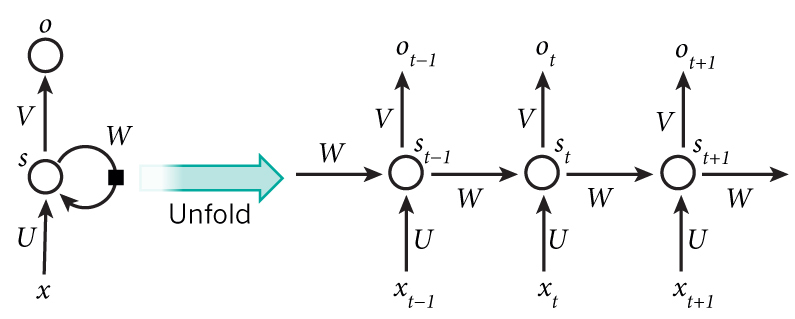
\includegraphics[width=13cm,height=5cm]{img/rnn}
     \caption[Architecture of RNN]{Architecture of RNN \cite{rnnintro}}
     \label{rnn}
\end{center}
\end{figure}
The Figure \ref{rnn} shows a RNN being unrolled (or unfolded) into a full network. By unrolling we simply mean that we write out the network for the complete sequence.

As we can see form Table \ref{imagelabelcompare}, Inception-ResNet provides top-5 error rate of 3.7\% which is even less than average 5\% error rate of human. So we can say that Inception-ResNet provides best accuracy for image labeling task. \\

Similarly for image captioning task previous state of the art model im2text is unable to generate new caption due to its architecture. This problem is solved by Show and Tell(NIC) model. Comparison of both is given in table below.
\begin{table}[H]
\caption{Comparison of different image captioning models}
\label{imagecaptioncompare}
\begin{centering}
\begin{tabular}{|c|c|}
\hline
\textbf{Approch} & \textbf{BLEU Score}\tabularnewline
\hline
\hline
Im2Text \cite{ordonez2011im2text} & 11\tabularnewline
\hline
Show and Tell \cite{7505636} & 28\tabularnewline
\hline
\end{tabular}
\par\end{centering}

\end{table}

In Table \ref{imagecaptioncompare} BLEU score denotes how natural generated sentence is with compared to reference sentence. It is also dependent on sentences used for used for calculating BLEU score so average of multiple BLEU score for same model is used. 
\flushbottom
%%-------------------------------------------------------------------------

%%-------------------------------------------------------------------------
% ----Conclusion and Future Work---------
\flushbottom
\chapter{Conclusion and Future Work}\label{Conclusion and Future Work}
\section{Conclusion}
%Being able to automatically describe the content of an
%image using properly formed English sentences is a
%very challenging task, but it could have great impact, for
%instance by helping visually impaired people better understand
%the content of images on the web. The description must capture not only the objects contained in
%an image, but it also must express how these objects relate to
%each other as well as their attributes and the activities they
%are involved in. Moreover, the above semantic knowledge
%has to be expressed in a natural language like English, which
%means that a language model is needed in addition to visual
%understanding.

Combining recent advancement in Image Labeling and Automatic Machine Translation, an end-to-end hybrid neural network system is created. This system is capable to autonomously view an image and generate a reasonable description in natural language. Using Inception-ResNet provides better accuracy in identifying objects in image while LSTM will help us to relate that objects and create meaningful sentence.

\section{Future work}

In next phase, we will implement hybrid model as mentioned in our proposed plan. We will use ImageNet dataset for training newly added Inception-Resnet model. To complete training of our proposed approach, we will use MSCOCO dataset and then fine tune Inception-ResNet to achieve more accuracy. Once done with optimization, intuitive interface for user will be implemented, where user can easily upload images and generate captions. Multicore GPUs and distributed training will also be used for fast and efficient results.
%In order to speedup process of training and execution, we are also planing to take help of multicore GPUs and distributed training.

\flushbottom

%------------ Appendix ----------------
\flushbottom
\appendix
%\include{AppendixA}
\flushbottom
%%-------------------------------------------------------------------------
%-----------------publication---------------------------------------
%\flushbottom
%\chapter{List of publication}\label{publication}
%\begin{enumerate}[1.]
%  \item {Purvi Tandel, Sharada Valiveti, K P Agrawal and K. Kotecha: \textbf{"Non-repudiation in Ad Hoc Networks"},The 2010 International Conference on Future Generation Communication and Networking- MANET 2010, on December 13-15, 2010 in International Convention Center Jeju , Jeju Island, Korea, Communications in Computer and Information Science, 2010, Volume 120, pp. 405-415, (2010).}
%  \item {Paper titled  \textbf{"Witness Selection to Achieve Non-repudiation in Ad-hoc Networks"} selected in the 2011 International Conference on Wireless and Optical Communications, may 21-22, Zhengzhou, China. The conference proceeding will be published by IEEE press in IEEE Xplore.}
%\end{enumerate}
\begin{enumerate}
  \item {Purvi Tandel, Sharada Valiveti, K P Agrawal and K. Kotecha: \textbf{"Non-repudiation in Ad Hoc Networks"},The 2010 International Conference on Future Generation Communication and Networking- MANET 2010, on December 13-15, 2010 in International Convention Center Jeju , Jeju Island, Korea, Communications in Computer and Information Science, 2010, Volume 120, pp. 405-415, (2010).}
\end{enumerate}

%\flushbottom
%------------------------------------------------------------------------
% ------------ Bibliography---------------


\renewcommand{\bibname}{References}
\begin{singlespace}
\bibliographystyle{ieeetr}
\bibliography{reference}

%\begin{thebibliography}{50}
\addcontentsline{toc}{chapter}{REFERENCES}
%\bibitem[1]{ref1}{Zhou, L., Haas, Z.J.:"Securing Ad Hoc Networks", IEEE Network 13 (1999) 24–30.}
%\bibitem[2]{ref2}{Yu, S., Zhang, Y., Song, C., Chen, K.: "A security architecture for Mobile Ad Hoc Networks", Proceedings of Asia-Pasific Advanced Network(APAN), 2004.}
%\end{thebibliography}
\end{singlespace}

\end{document} 